\documentclass[11pt,a4paper]{article}
\usepackage[a4paper,margin=2.2cm]{geometry}
\usepackage{iftex}
\ifPDFTeX
  \usepackage[utf8]{inputenc}
  \usepackage[T1]{fontenc}
  \usepackage[spanish]{babel}
\else
  \usepackage{fontspec}
  \usepackage{polyglossia}
  \setmainlanguage{spanish}
  \setmainfont{Latin Modern Roman}
  \setsansfont{Latin Modern Sans}
  \setmonofont{Latin Modern Mono}
\fi
\usepackage{microtype}
\usepackage{amsmath}
\usepackage{graphicx}
\graphicspath{{../Figuras/}}
\usepackage{booktabs}
\usepackage{caption}
\usepackage{array}
\usepackage{tabularx}
\usepackage{enumitem}
\usepackage{xcolor}
\usepackage{hyperref}
\hypersetup{colorlinks=true, linkcolor=black, urlcolor=blue!60!black}
\usepackage{verbatim}
\usepackage{needspace}
\usepackage{titlesec}
\usepackage{setspace}
\setlist{nosep}
\setstretch{1.04}
\setlength{\parskip}{0.45ex plus 0.1ex minus 0.1ex}
\titlespacing*{\section}{0pt}{2ex plus 0.25ex minus 0.2ex}{0.9ex plus 0.15ex}
\titlespacing*{\subsection}{0pt}{1.5ex plus 0.2ex minus 0.2ex}{0.65ex plus 0.12ex}
\newcommand{\tfgrepo}{\url{https://github.com/Dafafi63f/Escape-Room.git}}
\newcommand{\bloquetfg}[1]{\par\smallskip\noindent #1\par}
\newcommand{\iniciotabla}{\par\medskip\renewcommand{\arraystretch}{1.12}}
\newcommand{\fintabla}{\par\medskip}

\title{Diseño y desarrollo de un juego interactivo educativo\\basado en contenidos del grado en Matemática Computacional y Análisis de Datos}
\author{%
  Daniel Fageda Figueredo \quad NIU: 1601846\\
  Tutor: Víctor Navas Portella
}
\date{}

\begin{document}
\maketitle

\noindent\textit{Nota sobre el título:} el documento de proyecto inicial planteaba un escape room con interfaz gráfica. El \textbf{entregable de este TFG} es el prototipo en consola (banco + tres modos de juego) descrito en esta memoria; la capa gráfica y narrativa queda como evolución futura del mismo proyecto.

\smallskip
\noindent El detalle técnico del repositorio (esquema del banco, scripts, arquitectura del juego) se documenta en los \texttt{README.md} del proyecto y se cita en los apéndices al final de esta memoria.

\smallskip
\noindent\textbf{Versión de entrega:} dos Word en \texttt{Entrega/Memoria/} (\texttt{Memoria\_TFG\_markdown.docx}, \texttt{Memoria\_TFG\_latex.docx}); figuras en \texttt{Entrega/Figuras/}. Regenerar figuras: \texttt{python Entrega/generar\_figuras\_memoria.py}. Regenerar Word: \texttt{python Entrega/exportar\_memoria.py}. El PDF de entrega lo exportas desde Word tras editar.

\begin{abstract}
\noindent Se presenta el diseño e implementación de un cuestionario educativo alineado con el plan de estudios del grado en Matemática Computacional y Análisis de Datos (MatCAD). El entregable incluye un banco cerrado de \textbf{480 preguntas} con metadatos curriculares, un juego en consola con tres modos (libre, historia y feedback) y herramientas de validación del dataset. El documento de proyecto inicial planteaba un escape room con interfaz gráfica; se adoptó un enfoque incremental que prioriza el contenido evaluable y el motor de juego antes de la capa narrativa visual. Los resultados muestran un sistema funcional, documentado y extensible; la validación con usuarios y la interfaz gráfica quedan como trabajo futuro.

\medskip
\noindent\textbf{Palabras clave:} cuestionario educativo, gamificación, banco de preguntas, autoevaluación, MatCAD, serious games.
\end{abstract}

\section{Introducción}

\subsection{Contexto}

El grado en Matemática Computacional y Análisis de Datos (MatCAD) de la Universitat Autònoma de Barcelona articula un plan de estudios amplio en el que conviven contenidos de matemáticas, computación, estadística, optimización e inteligencia artificial. La evaluación continua y la autoevaluación son piezas habituales del aprendizaje universitario. Muchas herramientas genéricas de práctica (listas de ejercicios, plataformas de preguntas sin metadatos curriculares) \textbf{no etiquetan} el contenido según curso, semestre o asignatura del grado; ello dificulta practicar de forma segmentada alineada con el plan de estudios, sin que ello implique que los recursos institucionales del grado sean inadecuados.

Paralelamente, la gamificación y los \textit{serious games} (Michael y Chen, 2005) han ganado relevancia como complemento a la enseñanza formal: permiten practicar con retroalimentación inmediata y pueden favorecer la motivación mediante mecánicas de juego (vidas, puntuación, progresión), según evidencia en contextos educativos digitales (Kiili, 2005; Habgood y Ainsworth, 2011). Los escape rooms educativos y las novelas gráficas interactivas representan un subconjunto de los \textit{serious games} en el que la \textbf{narrativa} ---secuencia de escenas o salas que contextualizan los retos--- envuelve desafíos cognitivos; sin embargo, su desarrollo completo exige un esfuerzo considerable en diseño gráfico, guion y validación pedagógica.

\subsection{Motivación}

Este Trabajo de Fin de Grado surge de la necesidad de disponer de una herramienta de autoevaluación alineada con las asignaturas del grado. El sistema debe gestionar un banco de preguntas \textbf{estructurado y auditable} ---mediante reglas automatizadas, revisión manual documentada y scripts de mantenimiento reproducibles---, ofrecer una experiencia de juego que incentive la práctica repetida, permitir analizar la calidad del contenido (distractores, duplicados, coherencia curricular) y sentar las bases para modelos pedagógicos más ricos.

En este contexto, \textbf{gamificación} designa el uso de elementos de diseño de juego (puntos, vidas, retos, progresión) en un contexto formativo no recreativo (Deterding et al., 2011); en este TFG se aplica al cuestionario en consola sin interfaz gráfica. Un \textbf{banco de preguntas auditable} es un conjunto de ítems cuya calidad puede revisarse de forma sistemática mediante \texttt{mantenimiento.py validar}, la revisión manual (\texttt{Revision/revision\_manual\_banco.md}) y scripts de auditoría. Los \textbf{distractores plausibles} son opciones incorrectas creíbles para quien no domina el concepto (Haladyna et al., 2002). La \textbf{narrativa} (capa pendiente) sería la secuencia ficcional de escenas que contextualiza los retos; el entregable actual funciona sin ella. Por \textbf{multiasignatura} y \textbf{prerrequisitos} se entiende el solapamiento entre materias y los conocimientos previos que un ítem da por asumidos.

La motivación principal es combinar programación, matemáticas y diseño interactivo en una aplicación práctica que consolide conocimientos del grado y que pueda ser extendida por el propio autor o por el profesorado.

\subsection{Alcance del entregable}

El documento de proyecto inicial planteaba un juego interactivo tipo escape room con interfaz gráfica. Durante el desarrollo se priorizó la \textbf{calidad y estructura del banco de preguntas} y un \textbf{prototipo jugable en consola}, decisión metodológica coherente con un enfoque incremental: primero validar el contenido y la lógica de evaluación; después añadir la capa narrativa y gráfica.

\subsection{Objetivos derivados del desarrollo}

Durante el proyecto surgieron objetivos técnicos no recogidos en el documento inicial pero necesarios para la calidad del entregable: definir un \textbf{esquema canónico} del banco (480 preguntas, balance por dificultad, tipo y respuesta correcta), enriquecer cada pregunta con \textbf{metadatos curriculares} (curso, semestre, grupo temático, nivel), construir un \textbf{pipeline de mantenimiento} (validación, auditoría de distractores, deduplicación) e implementar un \textbf{modo historia} que genere exámenes balanceados según el histórico de calificaciones del grado (\texttt{Historic\_qualificacions\_MatCAD\_completo.csv}).

\subsection{Marco teórico y estado del arte}

\subsubsection{Aprendizaje activo y evaluación formativa}

El aprendizaje universitario de calidad se asocia a estrategias centradas en el estudiante (Biggs, Tang y Kennedy, 2022). La \textbf{evaluación formativa} orienta el aprendizaje (Nicol y Macfarlane-Dick, 2006). Los cuestionarios de opción múltiple exigen distractores plausibles (Haladyna et al., 2002).

\subsubsection{Gamificación, serious games y narrativa}

El \textit{game-based learning} ofrece retroalimentación inmediata (Prensky, 2003; Gee, 2003). Los \textit{serious games} (Michael y Chen, 2005) y escape rooms (Veldkamp et al., 2020) aportan narrativa; si no está alineada, puede distraer (Habgood y Ainsworth, 2011). Este TFG separa banco + motor de la narrativa gráfica pendiente.

\subsubsection{Posicionamiento}

Contribución: alineación curricular (40 materias, 4×2×5), trazabilidad de calidad del banco y arquitectura extensible. Los distractores \textbf{fuertes} son plausibles; los \textbf{débiles} delatan el ítem (auditoría + revisión manual).

\section{Objetivos}

\subsection{Objetivo general}

Diseñar e implementar un juego interactivo educativo en el que la progresión del jugador dependa de la resolución de retos basados en contenidos del grado en Matemática Computacional y Análisis de Datos.

\subsection{Objetivos específicos}

{\small\setlength{\tabcolsep}{4pt}%
\begin{tabular}{@{}l>{\raggedright\arraybackslash}p{3.4cm}>{\raggedright\arraybackslash}p{7.8cm}@{}}
\toprule
\textbf{\#} & \textbf{Objetivo} & \textbf{Indicador de logro} \\
\midrule
OE1 & Diseñar una narrativa interactiva como marco de los retos & Guion de escenas/salas vinculadas a materias del grado \\
OE2 & Crear distintos tipos de retos relacionados con las materias & Banco con preguntas de Teoría y Cálculo, tres niveles de dificultad, 40 materias \\
OE3 & Implementar algoritmos que validen las respuestas del jugador & Motor de partida con corrección A--D, puntuación, vidas, informes \\
OE4 & Desarrollar una interfaz gráfica sencilla e intuitiva & Interfaz gráfica de usuario (Pygame u otro motor) \\
OE5 & Evaluar el funcionamiento y el valor formativo del sistema & Banco validado, pruebas unitarias, revisión manual, modo feedback \\
\bottomrule
\end{tabular}}

\bloquetfg{El grado de cumplimiento de cada objetivo se discute en la sección~6.}

\section{Hipótesis de trabajo}

Hipótesis formuladas de modo \textbf{contrastable} con datos del sistema:

\textbf{H1.} Un banco estructurado según el plan curricular \textbf{permite autoevaluación segmentada} verificable con los filtros del modo libre.

\textbf{H2.} Un pipeline automatizado \textbf{detecta inconsistencias} (desequilibrios, distractores débiles, duplicados) con conteos reproducibles.

\textbf{H3.} El histórico de calificaciones \textbf{pondera materias} en el modo historia de forma coherente con estadísticas agregadas.

\begin{quote}
\textbf{Nota:} \textbf{H1}--\textbf{H2} con auditorías; \textbf{H3} con 8818 registros (§5.6). La motivación (gamificación vs.\ listado estático) queda en trabajo futuro (§6.6) por falta de datos de usuario.
\end{quote}

\section{Metodología}

\subsection{Enfoque general}

El desarrollo siguió una \textbf{metodología incremental} en cuatro fases, alineada con el documento de proyecto:
\begin{enumerate}
  \item \textbf{Análisis y diseño:} definición de materias, esquema del banco, metadatos y modos de juego.
  \item \textbf{Implementación:} dataset, scripts de mantenimiento, motor de partida en consola.
  \item \textbf{Pruebas:} validación estructural, pruebas unitarias, revisión manual del contenido.
  \item \textbf{Evaluación:} análisis del resultado, identificación de limitaciones y líneas futuras.
\end{enumerate}

El control de versiones con Git permitió iterar sobre el banco y el código de forma trazable. El repositorio público facilita la reproducibilidad del trabajo.

\subsection{Diseño del banco de preguntas}

\bloquetfg{\textbf{Población de ítems:} 40 materias del grado MatCAD × 12 preguntas = \textbf{480 ítems}.}

\bloquetfg{\textbf{Esquema por materia:} notación \texttt{2FT 2MT 2DT 2FC 2MC 2DC}, donde la letra indica \textbf{T}eoría o \textbf{C}álculo y la inicial \textbf{F}ácil, \textbf{M}edia o \textbf{D}ifícil (p.\ ej.\ \texttt{2FT} = dos preguntas de Teoría Fácil). En total: 6 de Teoría + 6 de Cálculo, con escalón Fácil → Media → Difícil en cada mitad.}

\bloquetfg{\textbf{Reparto global:}}
\iniciotabla
\begin{tabular}{@{}ll@{}}
\toprule
\textbf{Dimensión} & \textbf{Distribución} \\
\midrule
Dificultad & 160 Fácil / 160 Media / 160 Difícil \\
Tipo & 240 Teoría / 240 Cálculo \\
Respuesta correcta & 120 por letra A, B, C y D \\
\bottomrule
\end{tabular}
\fintabla

\bloquetfg{\textbf{Metadatos curriculares} en \texttt{listado\_materias.csv}: \texttt{Grupo}, \texttt{Nivel}, \texttt{Curso}, \texttt{Semestre}, \texttt{Tematica} (10 grupos temáticos globales).}

\bloquetfg{\textbf{Revisión de contenido:} revisión manual por bloques de Ids (1--480), con registro en \texttt{Revision/revision\_manual\_banco.md}. Criterios: redacción genérica, coherencia con el nivel de la materia, distractores plausibles, ausencia de referencias a temarios internos de asignatura.}

\bloquetfg{\textbf{Validación automatizada:} comando \texttt{mantenimiento.py validar} comprueba balance, orden canónico e integridad de columnas. Auditoría de distractores y detección de duplicados semánticos mediante scripts dedicados.}

\bloquetfg{Detalle técnico: \texttt{Data/README.md}.}

\subsection{Diseño e implementación del software}

\textbf{Stack tecnológico:}
\begin{itemize}
  \item Lenguaje: Python 3.10+ (biblioteca estándar en el juego; sin dependencias externas obligatorias).
  \item Persistencia: CSV y JSON para datos; informes y feedback en \texttt{.txt} locales.
  \item Empaquetado opcional: PyInstaller (Windows), script \texttt{build\_exe\_onefile.ps1}.
\end{itemize}

La arquitectura del software se organiza en capas desacopladas (figura~\ref{fig:arquitectura}): el lanzador orquesta los modos de juego; cada modo delega en el motor de partida la corrección, la puntuación y los informes; la capa de datos abstrae el acceso al banco cerrado y a los metadatos curriculares. Los scripts de mantenimiento operan sobre los mismos ficheros sin formar parte del ejecutable del juego.

\begin{figure}[htbp]
\centering

\includegraphics[width=0.92\linewidth]{arquitectura_sistema.png}
\caption{Arquitectura en capas del cuestionario MATCAD (módulos principales y flujo de dependencias).}
\label{fig:arquitectura}
\end{figure}

\iniciotabla
\begin{tabularx}{\linewidth}{@{}>{\raggedright\arraybackslash}p{2.1cm}>{\raggedright\arraybackslash}p{5.4cm}>{\raggedright\arraybackslash}X@{}}
\toprule
\textbf{Capa} & \textbf{Módulos} & \textbf{Función} \\
\midrule
Lanzador & \texttt{juego\_cuestionario.py} & Menú, tutorial de teclado, bucle de modos \\
Modos & \texttt{modo\_libre.py}\newline\texttt{modo\_historia.py}\newline\texttt{modo\_feedback.py} & Flujos pedagógicos distintos \\
Motor & \texttt{motor\_partida.py}\newline\texttt{reglas\_partida.py}\newline\texttt{politica\_reglas.py} & Preguntas, vidas, puntuación, informes \\
Datos & \texttt{datos.py}\newline\texttt{modelos.py}\newline\texttt{rutas.py} & Carga CSV/JSON, metadatos, rutas \\
Interacción & \texttt{consola.py}\newline\texttt{entrada\_menu.py}\newline\texttt{navegacion.py} & Teclas, menús, pausa, ayuda \\
Historia & \texttt{generador\_examen\_historia.py} & Ponderación según histórico de calificaciones \\
\bottomrule
\end{tabularx}
\fintabla

\bloquetfg{\textbf{Modos implementados:}}
\iniciotabla
\begin{tabular}{@{}lp{9cm}@{}}
\toprule
\textbf{Modo} & \textbf{Función pedagógica} \\
\midrule
\textbf{Libre} & Autoevaluación abierta con filtros por curso, semestre, temática, grupo, nivel, materia y dificultad \\
\textbf{Historia} & Simulación de examen balanceado según histórico de qualificacions del grado \\
\textbf{Feedback} & Canal de mejora continua (bugs, sugerencias) hacia el creador \\
\bottomrule
\end{tabular}
\fintabla

\bloquetfg{\textbf{Evaluación del jugador} (\texttt{motor\_partida.py}): cada respuesta A--D se compara con el campo \texttt{Correcta}.}
\iniciotabla
\begin{tabular}{@{}lp{9.5cm}@{}}
\toprule
\textbf{Mecanismo} & \textbf{Comportamiento} \\
\midrule
Corrección inmediata & Acierto/fallo con feedback; modo examen sin pistas hasta el informe final. \\
Puntuación arcade & +10/+20/+30 (F/M/D); penalización $\geq 5$ o mitad del valor base. \\
Nota & $10 \times \text{aciertos}/\text{total}$ en presets NOTA/PORCENTAJE. \\
Vidas & 3 por defecto; error resta una vida; partida termina a 0. \\
Progresión & Dificultad global sube cada 3 preguntas (modo libre arcade). \\
\bottomrule
\end{tabular}
\fintabla

\subsection{Validación y aseguramiento de la calidad}

\iniciotabla
\begin{tabular}{@{}lp{8cm}@{}}
\toprule
\textbf{Actividad} & \textbf{Herramienta / método} \\
\midrule
Balance estructural del CSV & \texttt{mantenimiento.py validar} \\
Revisión manual del contenido & Bloques documentados en \texttt{Revision/revision\_manual\_banco.md} \\
Auditoría de distractores & \texttt{mantenimiento.py auditar-distractores} (consola; \texttt{--json} opcional) \\
Duplicados semánticos & \texttt{duplicados.py revisar} \\
Pruebas de regresión del juego & \texttt{python -m unittest discover -s Juego/Tests -v} \\
Revisión con profesorado & Identificación de solapamiento temático y prerrequisitos (véase sección 8) \\
Simulación Monte Carlo (respuestas al azar) & \texttt{simulacion\_evaluacion\_azar.py} (véase \S\,5.7) \\
\bottomrule
\end{tabular}
\fintabla

El banco de producción (\texttt{Preguntas.csv}) se declaró \textbf{cerrado} en junio de 2026; las escrituras en el CSV requieren \texttt{TFG\_PERMITIR\_CSV=1} para evitar modificaciones accidentales.

\subsection{Criterios de éxito}

Se consideró exitoso el entregable si:
\begin{enumerate}
  \item El banco cumplía el esquema 480 ítems con balance verificado.
  \item Los tres modos de juego eran ejecutables sin errores en el flujo principal.
  \item Existía documentación reproducible (README, memoria, scripts de mantenimiento).
  \item El contenido había pasado revisión manual completa.
\end{enumerate}

\section{Resultados}

\subsection{Banco de preguntas}

Se obtuvo un banco cerrado de \textbf{480 preguntas} con las siguientes propiedades verificadas:
\begin{itemize}
  \item \textbf{40 materias} alineadas con el listado del grado.
  \item \textbf{12 preguntas por materia} siguiendo el patrón 2FT 2MT 2DT 2FC 2MC 2DC.
  \item \textbf{Revisión manual 480/480} completada en cinco tramos temporales.
  \item \textbf{Auditorías de calidad} ejecutadas (\texttt{mantenimiento.py auditar-distractores}, \texttt{duplicados.py revisar}): detección de pares similares pendientes de sustitución (3 en CSV modo seguro, $\sim$13 intra-materia en plantillas beta).
\end{itemize}

El banco distingue \textbf{modo seguro} (solo dataset revisado) y \textbf{modo beta} (pool ampliado con plantillas no revisadas, hasta 1440 ítems jugables), dejando clara la trazabilidad para evaluación formal del TFG.

\subsection{Aplicación de juego}

\textbf{Estado del entregable:} cuestionario en consola con tres modos operativos (libre, historia, feedback), banco de \textbf{480 preguntas} revisadas manualmente, herramientas de mantenimiento del dataset y empaquetado opcional en ejecutable Windows. La capa gráfica escape room / novela queda como evolución futura. \textbf{No se ha utilizado Pygame ni otro motor gráfico} en esta versión; la interfaz es exclusivamente textual en terminal.

Se entregó un cuestionario en consola funcional:

\begin{tabular}{@{}lp{8cm}@{}}
\toprule
\textbf{Componente} & \textbf{Resultado} \\
\midrule
Lanzador & \texttt{Juego/juego\_cuestionario.py} (tutorial de foco de teclado al inicio) \\
Paquete de lógica & \texttt{Juego/Consola/} (18 módulos) \\
Modo libre & Filtros multidimensionales, informes \texttt{.txt} \\
Modo historia & Generador de examen según \texttt{Historic\_qualificacions\_MatCAD\_completo.csv} \\
Modo feedback & Guardado local + envío SMTP opcional \\
Ejecutable & Build opcional con PyInstaller \\
Pruebas & Suite en \texttt{Juego/Tests/} (informes, entrada, feedback, configuración) \\
\bottomrule
\end{tabular}

\subsection{Organización curricular modelada}

Las 40 materias se distribuyen en \textbf{4 cursos × 2 semestres × 5 materias} (tabla~\ref{tab:curso-sem}). Los metadatos provienen de \texttt{listado\_materias.csv}.

\iniciotabla
\begin{tabular}{@{}ccc@{}}
\toprule
\textbf{Curso} & \textbf{Semestre 1} & \textbf{Semestre 2} \\
\midrule
1 & 5 & 5 \\
2 & 5 & 5 \\
3 & 5 & 5 \\
4 & 5 & 5 \\
\bottomrule
\end{tabular}
\captionof{table}{Materias por curso y semestre (5 por celda, 40 en total).}
\label{tab:curso-sem}
\fintabla

Transversalmente, las materias se agrupan en \textbf{10 grupos temáticos} (tabla~\ref{tab:grupos}). El grupo no coincide con el curso: varias materias del mismo bloque temático se imparten en etapas distintas del grado.

{\small\iniciotabla
\begin{tabular}{@{}clp{5.8cm}@{}}
\toprule
\textbf{Gr.} & \textbf{Mat.} & \textbf{Temática (resumen)} \\
\midrule
G1 & 2 & Álgebra y geometría / visualización \\
G2 & 5 & Cálculo y ecuaciones \\
G3 & 4 & Sistemas y seguridad computacional \\
G4 & 2 & Programación de software \\
G5 & 4 & Algoritmia y teoría de juegos \\
G6 & 4 & Métodos numéricos y optimización \\
G7 & 8 & Probabilidad y ciencia de datos \\
G8 & 3 & Bases de datos \\
G9 & 4 & Inteligencia artificial y aprendizaje automático \\
G10 & 4 & Modelización física e información \\
\bottomrule
\end{tabular}
\captionof{table}{Grupos temáticos y número de materias.}
\label{tab:grupos}
\fintabla}

Cada pregunta se enriquece al cargar con \texttt{curso}, \texttt{semestre}, \texttt{grupo}, \texttt{nivel} y \texttt{tematica}, lo que habilita filtros de partida alineados con la etapa formativa del estudiante.

Diagrama detallado (40 materias): \texttt{Data/README.md}.

\subsection{Herramientas de mantenimiento}

Se desarrolló un conjunto de scripts en \texttt{Files/Scripts/} con punto de entrada unificado (\texttt{mantenimiento.py}): validación, revisión, pipeline de plantillas, auditorías (salida en consola), deduplicación y estadísticas del histórico de qualificacions. Los scripts de regeneración masiva del CSV se aislaron en \texttt{Files/Archivo/} con protección de banco cerrado. Catálogo de comandos: \texttt{Files/Scripts/README.md}.

\subsection{Síntesis cuantitativa}

\begin{tabular}{@{}ll@{}}
\toprule
\textbf{Métrica} & \textbf{Valor} \\
\midrule
Preguntas en banco de producción & 480 \\
Materias cubiertas & 40 \\
Módulos Python del juego (Consola) & 18 \\
Modos de juego operativos & 3 \\
Pruebas unitarias & 4 módulos de test \\
Grupos temáticos modelados & 10 \\
\bottomrule
\end{tabular}

\subsection{Validación analítica del modo historia (H3)}

La hipótesis H3 se contrasta con el histórico institucional \texttt{Historic\_qualificacions\_MatCAD\_completo.csv} (\textbf{8818} registros de calificaciones), del que se derivan estadísticas agregadas por asignatura para las \textbf{40} materias del listado del grado.

El procedimiento, implementado en \texttt{generador\_examen\_historia.py}, sigue el flujo de la figura~\ref{fig:flujo-historia}. En primer lugar, por cada materia se calculan la media numérica, la tasa de suspensos (nota $< 5$) y un \textbf{índice de dificultad} en el intervalo $[0,1]$ que combina ambos indicadores. A continuación, el generador asigna \textbf{pesos} a las materias según el perfil elegido ---por ejemplo, el perfil \textit{refuerzo} incrementa el peso de las materias con índice alto---. Finalmente, por cada materia seleccionada se rellenan los \textit{slots} canónicos Teoría/Cálculo $\times$ Fácil/Media/Difícil con preguntas del banco cerrado.

\begin{figure}[htbp]
\centering
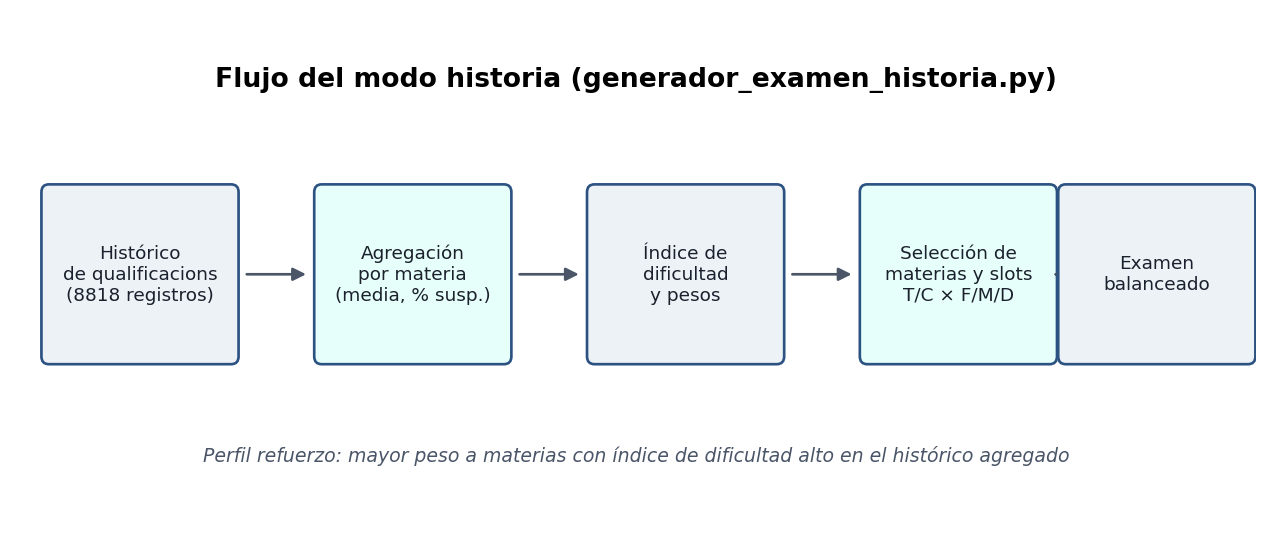
\includegraphics[width=0.95\linewidth]{flujo_modo_historia.png}
\caption{Pipeline del generador de examen balanceado (modo historia).}
\label{fig:flujo-historia}
\end{figure}

\iniciotabla
\begin{tabular}{@{}lrrrr@{}}
\toprule
\textbf{Materia} & \textbf{Índice} & \textbf{Media} & \textbf{\% susp.} & \textbf{Reg.} \\
\midrule
Càlcul en Diverses Variables & 0,026 & 5,66 & 22,9 & 341 \\
Probabilitat & 0,021 & 5,65 & 21,6 & 343 \\
Anàlisi Complexa i de Fourier & 0,008 & 5,55 & 16,3 & 258 \\
\bottomrule
\end{tabular}
\captionof{table}{Materias con mayor índice de dificultad en el histórico agregado (muestra ilustrativa).}
\label{tab:h4-dificultad}
\fintabla

Estos valores orientan la ponderación del modo historia; un piloto con estudiantes permitiría contrastar si los exámenes generados se perciben alineados con la exigencia real del grado.

\subsection{Simulación Monte Carlo (respuestas al azar)}

Para validar que el motor de corrección penaliza el azar como cabría esperar en un examen tipo test, se implementó \texttt{simulacion\_evaluacion\_azar.py} y se formalizó el experimento en términos probabilísticos. En cada ítem, la respuesta del jugador que contesta al azar se modela como una variable de Bernoulli $X_i \sim \mathrm{Bernoulli}(p)$ con $p = 1/4$, al elegir uniformemente entre las cuatro opciones A--D. El número de aciertos en un bloque de $n = 20$ preguntas es entonces
\[
Y = \sum_{i=1}^{n} X_i \sim \mathrm{Binomial}(n,\, p),
\]
con valor esperado $\mathbb{E}[Y] = np = 5$ y varianza $\mathrm{Var}(Y) = np(1-p) = 3{,}75$. La nota del motor, definida como $\mathrm{nota} = 10\,Y/n$, verifica $\mathbb{E}[\mathrm{nota}] = 2{,}5$, coherente con el umbral de suspensión universitario.

El estimador Monte Carlo de la fracción de aciertos tras $N$ réplicas independientes,
\[
\hat{p}_N = \frac{1}{N}\sum_{k=1}^{N}\frac{Y^{(k)}}{n},
\]
es insesgado ($\mathbb{E}[\hat{p}_N] = p$) y su error estándar decrece como $\mathcal{O}(1/\sqrt{N})$. Con $N = 50\,000$ y semilla 42, la simulación arroja una fracción media de \textbf{24,98\,\%}, próxima al valor teórico (figura~\ref{fig:mc-convergencia}). La figura~\ref{fig:mc-histograma} contrasta el histograma empírico de notas con la masa de probabilidad binomial.

\begin{figure}[htbp]
\centering

\includegraphics[width=0.98\linewidth]{monte_carlo_histograma_notas.png}
\caption{Histograma de la simulación (50\,000 réplicas) frente a la distribución binomial teórica.}
\label{fig:mc-histograma}
\end{figure}

\begin{figure}[htbp]
\centering
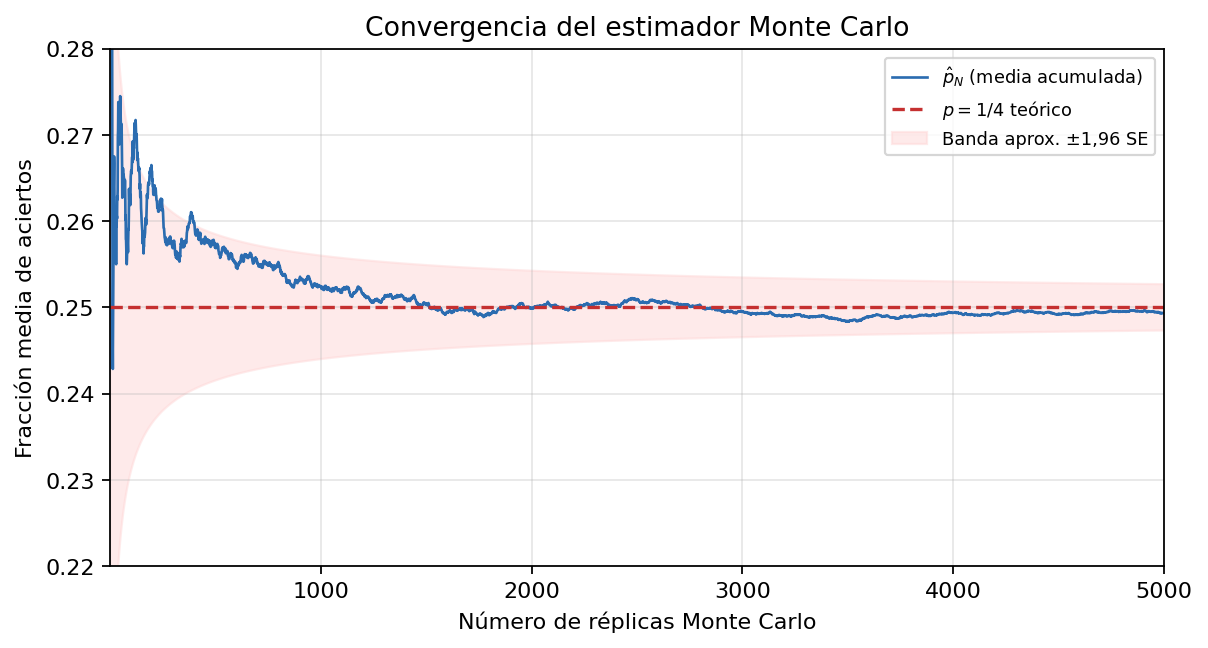
\includegraphics[width=0.88\linewidth]{monte_carlo_convergencia.png}
\caption{Convergencia de $\hat{p}_N$ hacia $p = 1/4$ al aumentar el número de réplicas.}
\label{fig:mc-convergencia}
\end{figure}

En el \textbf{modo arcade} con tres vidas, cada fallo consume una vida y la probabilidad de error por pregunta es $q = 3/4$. El número de preguntas respondidas hasta agotar las vidas coincide, en ausencia de límite superior, con el número de ensayos hasta observar $r = 3$ fallos en ensayos de Bernoulli con probabilidad de «éxito» $q$; dicha variable sigue una ley binomial negativa con valor esperado $\mathbb{E}[T] = r/q = 4$, lo que explica la media empírica de \textbf{4,0} preguntas por partida. La probabilidad de completar las 20 preguntas sin perder las tres vidas es $\mathbb{P}(Y_{20} \geq 18) = \sum_{j=18}^{20}\binom{20}{j}(1/4)^j(3/4)^{20-j}$, prácticamente nula; de ahí que el \textbf{100\,\%} de partidas simuladas agoten vidas antes del objetivo.

\iniciotabla
\begin{tabular}{@{}ll@{}}
\toprule
\textbf{Escenario} & \textbf{Resultado} \\
\midrule
Modo examen: fracción media de aciertos & \textbf{24,98\,\%} \\
Modo examen: nota media /10 & \textbf{2,5} \\
Modo arcade: partidas que agotan vidas & \textbf{100\,\%} \\
Modo arcade: preguntas respondidas de media & \textbf{4,0} / 20 \\
Modo arcade: puntos medios & \textbf{$-10$} \\
\bottomrule
\end{tabular}
\captionof{table}{Resumen numérico de la simulación Monte Carlo (semilla 42).}
\label{tab:mc-resumen}
\fintabla

En conjunto, el experimento demuestra que el azar produce suspensión sistemática y que, con vidas limitadas, impide completar bloques largos sin conocimiento real. Las figuras se regeneran con \texttt{python Entrega/generar\_figuras\_memoria.py}; la simulación numérica, con \texttt{python Files/Scripts/simulacion\_evaluacion\_azar.py}.

\section{Discusión}

\subsection{Cumplimiento de los objetivos}

El \textbf{objetivo general} se cumple de forma parcial: existe un juego educativo interactivo basado en contenidos del grado, pero la progresión narrativa tipo escape room no está implementada. La progresión actual es ludificada (vidas, puntos, dificultad creciente) y curricular (filtros por etapa del grado).

\iniciotabla
\begin{tabular}{@{}llp{6.5cm}@{}}
\toprule
\textbf{\#} & \textbf{Estado} & \textbf{Comentario} \\
\midrule
OE1 & Pendiente (futuro) & Sin guion de escenas/salas implementado \\
OE2 & \textbf{Cumplido} & Banco 480 ítems, Teoría/Cálculo, tres dificultades \\
OE3 & \textbf{Cumplido} & Motor A--D, puntuación, vidas, informes \\
OE4 & Pendiente (futuro) & Solo consola; Pygame no utilizado \\
OE5 & \textbf{Parcialmente cumplido} & Banco validado y tests; sin estudio con usuarios \\
\bottomrule
\end{tabular}
\fintabla

Los \textbf{objetivos específicos} OE2, OE3 y OE5 están cubiertos en su versión de consola. OE1 y OE4 (narrativa gráfica e interfaz visual) quedan explícitamente como trabajo futuro. Esta decisión es defendible: el prototipo valida el núcleo evaluable sin el coste de desarrollo gráfico, en línea con el principio de prototipado incremental en ingeniería del software.

\subsection{Validez del banco de preguntas}

La \textbf{validez de contenido} se abordó mediante revisión manual exhaustiva y criterios de redacción acordados. La \textbf{validez estructural} se garantiza con reglas de balance automatizadas. Quedan abiertas:
\begin{itemize}
  \item la \textbf{validez semántica} fina (algunos pares de ítems muy similares),
  \item y la \textbf{validez predictiva} (relación entre desempeño en el juego y desempeño académico real), no medida en este TFG.
\end{itemize}

La revisión con profesorado puso de manifiesto limitaciones del modelo de una sola etiqueta \texttt{Materia}:
\begin{enumerate}
  \item \textbf{Solapamiento temático:} preguntas que encajan en varias asignaturas (p.\ ej.\ inferencia en Probabilidad y en Modelización e Inferencia).
  \item \textbf{Prerrequisitos:} preguntas de cursos avanzados que asumen conceptos de materias previas (p.\ ej.\ optimización y cálculo multivariable).
\end{enumerate}

Estas observaciones motivan la propuesta de campos \texttt{Materias\_relacionadas} y \texttt{Prerequisitos} en futuras versiones del esquema.

\subsection{Utilidad para autoevaluación y apoyo docente}

El sistema permite al estudiante practicar por \textbf{semestre o temática} acorde a su momento del grado, simular un \textbf{examen balanceado} mediante el modo historia y recibir un \textbf{informe detallado} al finalizar una partida en modo examen.

Para el profesorado, el banco estructurado y los scripts de auditoría facilitan revisión por materia y detección de ítems problemáticos. El modo feedback cierra un ciclo de mejora continua.

La interfaz en consola limita la accesibilidad para usuarios no familiarizados con terminal; el tutorial de foco de teclado al inicio mitiga parte de esa barrera, pero una GUI sería deseable para despliegue masivo.

\subsection{Relación con las hipótesis}

La hipótesis \textbf{H1} queda apoyada por la operatividad de los filtros curriculares en el modo libre, que permiten segmentar la práctica por curso, semestre y materia. \textbf{H2} se sustenta en las auditorías y en la validación estructural, cuyos conteos son reproducibles en cada ejecución de los scripts de mantenimiento. \textbf{H3} encuentra respaldo en el modo historia y en el análisis del histórico institucional (8818 registros), desarrollado en la sección~5.6. La simulación Monte Carlo de la sección~5.7 complementa estas hipótesis al verificar cuantitativamente que el motor de evaluación no concede aprobación al azar.

\subsection{Limitaciones del estudio}

El estudio no incluye \textbf{evaluación con usuarios}: no se recogieron datos de usabilidad ni de aprendizaje con una muestra de estudiantes. La \textbf{interfaz en consola} reduce el atractivo visual respecto al escape room planteado inicialmente. El \textbf{modelo de datos} asigna una sola materia por pregunta y aún no modela prerrequisitos explícitos. El \textbf{idioma del banco} mezcla castellano y catalán según la asignatura, con coherencia terminológica revisada pero mejorable. Por último, el \textbf{modo beta} amplía el pool con plantillas no revisadas y debe distinguirse del banco de producción en cualquier evaluación formal.

\subsection{Trabajo futuro}

Entre las líneas futuras inmediatas figuran la implementación de \texttt{Materias\_relacionadas} y \texttt{Prerequisitos} en el CSV y en los filtros del juego, el desarrollo de la capa gráfica escape room o novela gráfica, y la sustitución de pares de ítems semánticamente similares detectados por la auditoría. Conviene además contrastar si las mecánicas de juego aumentan la práctica respecto a un listado estático ---mediante un piloto con usuarios (n $\approx$ 15--20, cuestionario SUS, tiempo de práctica)---, línea no formulada como hipótesis contrastada en este TFG por ausencia de datos. La integración con plataformas institucionales (Moodle, AulaWeb) completaría el despliegue en el grado.

\section{Conclusiones}

Este Trabajo de Fin de Grado ha diseñado e implementado un \textbf{sistema de cuestionarios académicos} alineado con el plan de estudios del grado en Matemática Computacional y Análisis de Datos, integrando:
\begin{itemize}
  \item un \textbf{banco de 480 preguntas} estructurado, balanceado y revisado manualmente;
  \item un \textbf{juego en consola} con tres modos (libre, historia, feedback) que gamifica la autoevaluación;
  \item un \textbf{conjunto de herramientas} de validación y mantenimiento del dataset;
  \item y una \textbf{arquitectura extensible} preparada para narrativa gráfica y modelos pedagógicos más ricos.
\end{itemize}

La principal contribución académica es pasar de un cuestionario genérico a una herramienta con \textbf{criterio didáctico explícito}: trazabilidad curricular, calidad auditable del banco y mecánicas de juego orientadas a la práctica repetida. El desvío respecto al título inicial (escape room gráfico) se compensa con un entregable técnicamente sólido y documentado, que constituye la base sobre la que construir la experiencia narrativa.

En el plano personal, el proyecto ha consolidado competencias de programación en Python, diseño de datos, ingeniería de software incremental y reflexión pedagógica sobre la evaluación en grados STEM interdisciplinares.

Las líneas futuras más inmediatas son la validación con usuarios reales, el enriquecimiento del modelo de datos con multiasignatura y prerrequisitos, y el desarrollo de la interfaz gráfica prevista en el documento de proyecto.

\section{Bibliografía}

Biggs, J., Tang, C., y Kennedy, G. (2022). \textit{Teaching for Quality Learning at University} (5.ª ed.). McGraw-Hill Education (UK).

Brusilovsky, P., y Peylo, C. (2003). Adaptive and intelligent web-based educational systems. \textit{International Journal of Artificial Intelligence in Education}, \textit{13}(2--4), 159--172.

Deterding, S., Dixon, D., Khaled, R., y Nacke, L. (2011). From game design elements to gamefulness: Defining ``gamification''. En \textit{Proceedings of the 15th International Academic MindTrek Conference} (pp. 9--15). ACM. \url{https://doi.org/10.1145/2181037.2181040}

Gee, J. P. (2003). What video games have to teach us about learning and literacy. \textit{Computers in Entertainment}, \textit{1}(1), 20. \url{https://doi.org/10.1145/950566.950595}

Habgood, M. P. J., y Ainsworth, S. E. (2011). Motivating children to learn effectively: Exploring the use of intrinsic and extrinsic motivation in educational games. \textit{British Journal of Educational Technology}, \textit{42}(2), 183--200. \url{https://doi.org/10.1111/j.1467-8535.2009.01034.x}

Haladyna, T. M., Downing, S. M., y Rodriguez, M. C. (2002). A review of multiple-choice item-writing guidelines for classroom assessment. \textit{Applied Measurement in Education}, \textit{15}(3), 309--333. \url{https://doi.org/10.1207/S15324818AME1503_5}

Kiili, K. (2005). Digital game-based learning: Towards an experiential gaming model. \textit{The Internet and Higher Education}, \textit{8}(1), 13--24. \url{https://doi.org/10.1016/j.iheduc.2004.12.001}

Michael, D. R., y Chen, S. L. (2005). \textit{Serious Games: Games That Educate, Train, and Inform}. Thomson Course Technology.

Nicol, D. J., y Macfarlane-Dick, D. (2006). Formative assessment and self-regulated learning: A model and seven principles of good feedback practice. \textit{Studies in Higher Education}, \textit{31}(2), 199--218. \url{https://doi.org/10.1080/03075070600572090}

Prensky, M. (2003). Digital game-based learning. \textit{Computers in Entertainment}, \textit{1}(1), 21. \url{https://doi.org/10.1145/950566.950596}

Veldkamp, A., van de Grint, L., Knippels, M. C. P. J., y van Joolingen, W. R. (2020). Escape education: A systematic review on escape rooms in education. \textit{Educational Research Review}, \textit{31}, 100364. \url{https://doi.org/10.1016/j.edurev.2020.100364}

\section{Apéndices — documentación técnica del repositorio}
\renewcommand{\arraystretch}{1.08}
\begin{tabularx}{\textwidth}{@{}c>{\raggedright\arraybackslash}X>{\raggedright\arraybackslash}p{4.2cm}@{}}
\toprule
\textbf{Apéndice} & \textbf{Contenido} & \textbf{Enlace} \\
\midrule
A & Esquema del banco y diagramas curriculares & \texttt{Data/README.md} \\
H & Estado del proyecto y trazabilidad revisión manual (Ids 1--480) & \texttt{Revision/ESTADO.md}, \texttt{revision\_manual\_banco.md} \\
B & Arquitectura del juego, modos, puntuación, bancos beta & \texttt{Juego/Consola/README.md} \\
C & Scripts de mantenimiento, balanceo, auditorías & \texttt{Files/Scripts/README.md} \\
D & Scripts legado de regeneración CSV & \texttt{Files/Archivo/README.md} \\
E & Pruebas unitarias & \texttt{Juego/Tests/README.md} \\
F & Repositorio y guía rápida & \texttt{README.md} \\
G & LaTeX, Word y exportación & \texttt{Entrega/README.md} \\
\bottomrule
\end{tabularx}

\medskip
\noindent\textbf{Repositorio:} \tfgrepo

\end{document}
